\chapter{Notes from the Original Style Files\label{appendix_notes}}

These style-files for use with \LaTeX{} are maintained by Darrel
Hankerson\footnote{Mathematics and Statistics, 221 Parker Hall,
844-3641, {\tt hankedr@auburn.edu}} and Ed
Slaminka\footnote{Mathematics and Statistics, 218 Parker,
{\tt slamiee@auburn.edu}}. 

In 1990, department heads and other representatives met with Dean Doorenbos
and Judy Bush-Crofton (then responsible for manuscript approval). This
meeting was prompted by a memorandum\footnote{Originally, the memorandum
was presented to Professor Larry Wit. A copy is available on request.} from
members of the mathematics departments concerning the {\em Thesis and
Dissertation Guide\/} and the approval process. There was wide agreement
among the participants (including Dean Doorenbos) to support the basic
recommendations outlined in the memorandum. The revised {\em Guide\/}
reflected some (but not all) of the agreements of the meeting.

Ms Bush-Crofton was supportive of the plan to obtain ``official approval''
of these style files.\footnote{Followup memoranda gave a definition of
``official approval.'' Copies will be sent on request.}  Unfortunately, Ms
Bush-Crofton left the Graduate School before the process was completed. In
1994, we were revisiting some of the same problems which were
resolved at the 1990 meeting.

In Summer 1994, I sent several memoranda to Ms Ilga Trend of the Graduate
School, reminding her of the agreements made at the 1990 meeting.
Professors A. Scottedward Hodel and Stan Reeves provided additional
support.  In short, it is essential that the Graduate School honor its
commitments of the 1990 meeting. It should be emphasized that Dean
Doorenbos is to thank for the success of that meeting.

Maintaining these \LaTeX{} files has been more work than expected, in
part due to continuing changes in requirement by the graduate school.
The Graduate School occasionally has complete memory loss about the
agreements of the 1990 meeting. If the Graduate School rejects your
manuscript based on items controlled by the style-files, ask
your advisor to contact the Graduate school (and copy to the chair) to urge
cooperation.

Finally, there have been several requests for additions to the package
(mostly formatting changes for figures, etc.). While such changes are not
really part of the thesis-style package, it could be beneficial to collect
these options and distribute with the package (making it easier on the next
student).  I'm especially interested in changes needed by various
departments.


%%%%%%%%%%%%%%%%%%%%%%%%%%%%%%%%%%%%%%%%%%%%%%%%%%%%%%%%%%%%%%%%%%%%
% REMOVE THIS SECTION WHEN PREPARING YOUR OWN MANUSCRIPT AND WRITE %
%          THE FILES NEEDED TO MEET THE ABOVE ORGANIZATION         % 
%%%%%%%%%%%%%%%%%%%%%%%%%%%%%%%%%%%%%%%%%%%%%%%%%%%%%%%%%%%%%%%%%%%%

\chapter{The SUNY Poly Style Guide Chapter Name is so\\ 
         Long we Break it Over Multiple Lines\label{second}}  % Use \\ for long titles 

\section{Help with \LaTeX{}}

Your choice to use \LaTeX{}, specifically \LaTeX2e{}, to typeset your thesis will almost certainly 
benefit your manuscript; not only in appearance, but in your ability to edit,
organize, reorganize, and direct the content without worry or delay because of formatting.  Whether 
you are new to \LaTeX{} or an experienced user, it never hurts to have a solid tool set and reference
materials to support your work.  

The standard books on the subject are Lamport's \emph{\LaTeX{}: A Document Preparation System}
\cite{lamport_1994_latex} and Hahn's \emph{\LaTeX{} for Everyone} \cite{hahn_1993_latex}.
These seminal texts can be found in almost any academic library, but are regularly put on
hold and not really up to date.  Several fine introductions and references are available on the
Internet.  My favorite is \emph{A Simplified Introduction to {\LaTeX}} \cite{greenberg_2006_latex}.
This free book is particularly valuable for understanding the bibliography tool, Bibtex, 
basic mathematics typesetting, and counters.  \emph{The Not so Short Introduction to \LaTeX2e{}}
\cite{oetiker_2008_latex} is an excellent mathematics typesetting reference, 
and \emph{Getting Started with \LaTeX{}} \cite{wilkins_1995_latex} gets you into the basics of
\LaTeX{} typesetting quickly.

\section{Overleaf}
I highly recommend the online \LaTeX{} editor Overleaf \cite{overleafRef}.  It vastly simplifies the process of editing \LaTeX{} documents without necessarily having to install software locally.

\section{Supporting tools}

Whenever I use \LaTeX to typeset a document, I seem to find myself using the same supporting tools
again and again.  This section identifies the most common of these tools
along with resources that can be used to get started or as a reference.

\subsection{Make}
I always use {\tt make} to build my multifile documents.
The {\tt Makefile} provided with this document provides, among
others, {\tt all}, {\tt clean}, {\tt clean\_tex}, {\tt clean\_code}, and {\tt code}
targets, but most commonly you will use the command
\begin{center}
{\tt make}
\end{center}

As you create any new \LaTeX{} files you should add them to the {\tt TEXFILES} variable
to ensure proper builds.  If you have any code that produces \LaTeX{} files, or files 
included by other \LaTeX{} files, you will need to manage that through the 
{\tt Makefile.code} file you create.

\subsection{Aspell}

\emph{Aspell} is the replacement for the \emph{ispell} command line spell checker.  
This tool is useful in it's ability to check spelling inside \TeX{} and \LaTeX{}
source files.  It provides a menu driven, interactive shell that is very simple to use.
To check the spelling of a file called ``{\tt myfile.tex}'', enter the command
\begin{center}
{\tt aspell -c myfile.tex}
\end{center}

\subsection{Gnuplot}

\emph{Gnuplot} is a data visualization tool that can produce very clear Extended Postscript (EPS)
graphics in 2D and 3D from mathematical expressions and data files.  While Gnuplot can export 
to many graphic formats, EPS is one of the most common used in \LaTeX{} documents because
of the simple use of the {\tt epsfig} package.  Figure \ref{fig_gnuplot} 
is an example Gnuplot graph from my dissertation added to the document with {\tt epsfig}.  

\begin{figure}
\begin{center}
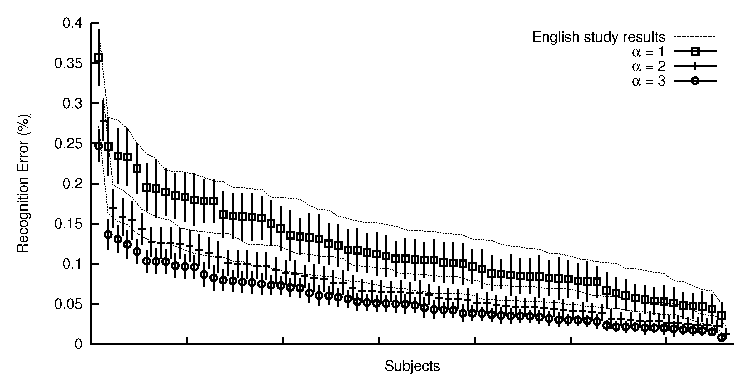
\epsfig{file=sample_gnuplot.eps, width=5in}
\caption{Example gnuplot graph included with the {\tt epsfig} package} 
\label{fig_gnuplot}
\end{center}
\end{figure}

%%%%%%%%%%%%%%%%%%%%%%%%%%%%%%%%%%%%%%%%%%%%%%%%%%%%%%%%%%%%%%%%%%%%
%                   STOP REMOVING HERE :-)                         %
%%%%%%%%%%%%%%%%%%%%%%%%%%%%%%%%%%%%%%%%%%%%%%%%%%%%%%%%%%%%%%%%%%%%



